\documentclass[aspectratio=169]{beamer}

\usetheme{Madrid}
\usecolortheme{beaver}
\usepackage{listings}
\usepackage{relsize}
\usepackage{ulem}

\setbeamertemplate{navigation symbols}{}

\hypersetup{
    colorlinks=true,
    linkcolor=darkred,
    filecolor=magenta,      
    urlcolor=darkred,
    pdftitle={GHC's JavaScript Backend},
    % pdfpagemode=FullScreen,
    }

\lstset{
  showstringspaces=false,
  stringstyle=\ttfamily\color{red},
  commentstyle=\ttfamily,
  keywordstyle=
}

\AtBeginSection[]
{
  \begin{frame}
    \frametitle{Table of Contents}
    \tableofcontents[currentsection]
  \end{frame}
}

\title{GHC's Optimizer}
\author{Sylvain HENRY}
\institute[IOG]{
\includegraphics[scale=0.2]{images/iohk-logo.png}}
\date[2023-08-10]{GHC DevX -- Learning Call\\10 August 2023}

\begin{document}

\frame{\titlepage}

%\begin{frame}
%\frametitle{Table of Contents}
%\tableofcontents
%\end{frame}

\begin{frame}
\frametitle{GHC's optimizations}

  \begin{itemize}
    \item Core optimizations
    \item STG optimizations
    \item Cmm optimizations
    \item Asm optimizations
  \end{itemize}

  We won't have time to fully cover everything. I'll only give an intuition and
  some references to learn more.
\end{frame}

\section{Core AST}

\begin{frame}[fragile]
  \frametitle{Core AST}
  \begin{columns}
    \begin{column}{0.55\textwidth}
      \begin{lstlisting}[language=haskell]
data Expr b
  = Var   Id
  | Lit   Literal
  | App   (Expr b) (Arg b)
  | Lam   b (Expr b)
  | Let   (Bind b) (Expr b)
  | Case  (Expr b) b Type [Alt b]
  | Cast  (Expr b) CoercionR
  | Tick  CoreTickish (Expr b)
  | Type  Type
  | Coercion Coercion
  \end{lstlisting}
    \end{column}
    \begin{column}{0.45\textwidth}
      \begin{onlyenv}<2>
      \small
      \begin{lstlisting}[language=haskell]
data Alt b
  = Alt AltCon [b] (Expr b)

data AltCon
  = DataAlt DataCon
  | LitAlt  Literal
  | DEFAULT

data Bind b
  = NonRec b (Expr b)
  | Rec [(b, (Expr b))]

type Id       = Var
data Var      = ...
data Coercion = ...
data Type     = ...
      \end{lstlisting}
    \end{onlyenv}
    \end{column}
  \end{columns}

  \begin{onlyenv}<1>
  References:
  \begin{itemize}
    \item 2022 - "Into the Core: Squeezing Haskell into \sout{9} 10 constructors" (SPJ)
  \end{itemize}
  \end{onlyenv}
\end{frame}

\begin{frame}[fragile]
  \frametitle{Rant: Core's 10 constructors}
  \begin{itemize}
    \item Could we have less than 10 constructors?
    \pause
     Yes! One constructor!
  \end{itemize}
  \begin{lstlisting}[language=haskell,basicstyle=\small]
  data Expr = Expr Dynamic -- contains a Core datacon, promise

  data Var = Var Id
  data Lit = Lit Literal
  ...
  \end{lstlisting}
  \pause
  \begin{itemize}
    \item Hey! You're cheating! You've lost type safety!
    \pause
    \item Yes, but it's already quite lost! Look at `Id` (IdDetails, IdInfo):
      \begin{itemize}
        \item We need shotgun parsing to handle ad-hoc cases:
        \begin{itemize}
          \item Primops, data-con workers \& wrappers, class ops, record
            selectors, covars, dfuns...
        \end{itemize}
        \item Sometimes they work the same, sometimes they don't. Good luck!
      \end{itemize}
    \pause
    \item Take-away: Core optimization in practice is much trickier than it looks (e.g. in papers)
    \begin{itemize}
      \item The compiler doesn't help much (cf shotgun parsing)
      \item E.g. it doesn't tell you that you forgot to handle `keepAlive\#` or
        `seq\#` primops properly in your optimization pass or analysis
        \begin{itemize}
          \item At best: missed optimization
          \item At worst: bug!
        \end{itemize}
    \end{itemize}
  \end{itemize}
\end{frame}

\section{Core optimizations}

\begin{frame}
  \frametitle{Core optimization pipeline}
  \begin{itemize}
    \item Pipeline stages (a.k.a. CoreToDo)
      \begin{itemize}
        \item Simplifier (many local transformations)
        \item Worker-wrapper
        \item Float-in and float-out
        \item Full-laziness
        \item + many other passes and analyses
      \end{itemize}
    \item Phases: initial ("gentle"), 2, 1, 0, final*
      \begin{itemize}
        \item Some rules and unfoldings (inlining) only enabled in some phases
        \item Users can only specify 0-2 in pragmas
        \item Final phase run repeatedly
      \end{itemize}
  \end{itemize}

  References:
  \begin{itemize}
    \item GHC.Core.Opt.Pipeline
    \item Note [Compiler phases] in GHC.Types.Basic
  \end{itemize}
\end{frame}

\begin{frame}
  \frametitle{Simple optimiser: simpler, alternative optimization pipeline}

  \begin{itemize}
    \item Performs:
      \begin{itemize}
        \item Occurrence analysis
        \item Beta-reduction
        \item Inlining
        \item Case of known constructor
        \item Dead code elimination
        \item Coercion optimisation
        \item Eta-reduction
        \item ... more? (documentation is terrible)
      \end{itemize}
    \item Used to simplify statically defined unfoldings, etc.
    \item Pure function: no stats, no dumps, etc.
    \item Do not confound "simple" with "simplifier"
  \end{itemize}

  References:
  \begin{itemize}
    \item GHC.Core.SimpleOpt
  \end{itemize}
\end{frame}

\begin{frame}
  \frametitle{Simplifier}
  \begin{itemize}
    \item Performs a bunch of local transformations
    \item Several simplifier iterations per phase of the optimization pipeline
      \begin{itemize}
        \item Until fixpoint or N iterations (4 by default, set with
          `-fmax-simplifier-iterations`)
      \end{itemize}
  \end{itemize}

  References:
  \begin{itemize}
    \item GHC.Core.Opt.Simplify.*
      \begin{itemize}
        \item "Utils" module contains optimizations too! e.g. see mkCase
      \end{itemize}
    \item 1995 - "Compilation by transformation in non-strict functional
      languages" (Santos' thesis)
  \end{itemize}
\end{frame}

\begin{frame}
  \frametitle{Simplifier: Santos' thesis 1/2}

  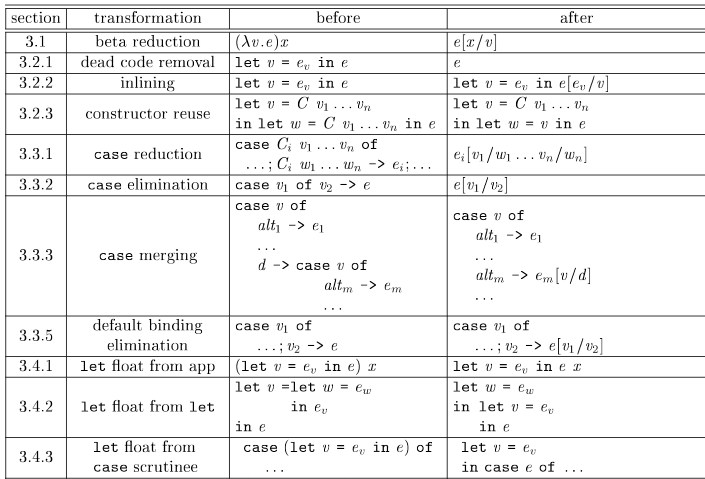
\includegraphics[width=25pc]{images/santos1.png}
\end{frame}

\begin{frame}
  \frametitle{Simplifier: Santos' thesis 2/2}

  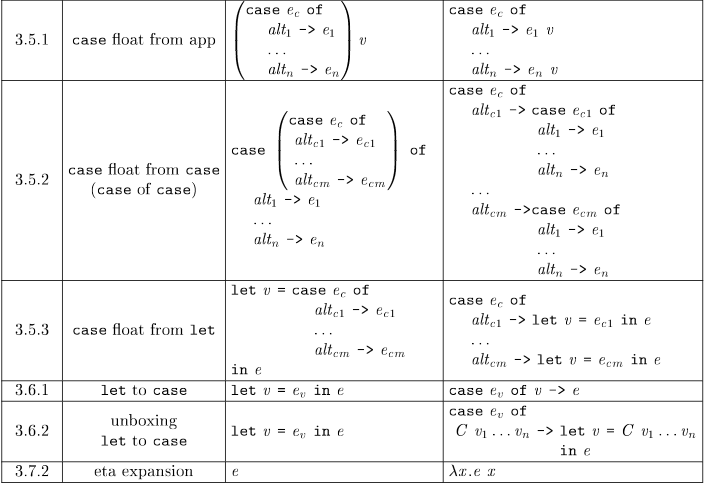
\includegraphics[width=25pc]{images/santos2.png}
\end{frame}

\begin{frame}
  \frametitle{Case of known constructor}
  \begin{itemize}
    \item Also called "case reduction" (Santos)
    \item case C a b of \{ ...; C x y $\rightarrow$ e ;... \} $\Longrightarrow$ e[a/x,b/y]
    \item Also applies to variable scrutinees which we know to be bound to a
      datacon
      \begin{itemize}
        \item case C a b of v \{ .. case v of ... C x y $\rightarrow$ e ...\}
        \item let v = C a b in .. case v of ... C x y $\rightarrow$ e ...
      \end{itemize}
    \item Made trickier by datacon wrappers that inline late... but for which we
      want to apply this optimization early
      \begin{itemize}
        \item Inline wrapper on the fly. Some wrinkles (see Notes)
      \end{itemize}
  \end{itemize}

  References:
  \begin{itemize}
    \item 1995 - "Compilation by transformation in non-strict functional
      languages" (Santos' thesis)
  \end{itemize}
\end{frame}

\begin{frame}
  \frametitle{Let-floating: float-in, float-out (full-laziness)}

  \begin{itemize}
    \item Float-in
      \begin{itemize}
        \item float let-bindings closer to their use sites
        \item reduce allocation scope
      \end{itemize}
    \item Float-out (full-laziness)
      \begin{itemize}
        \item float let-bindings towards the top-level
        \item allow other optimizations to fire (without lets in their way)
        \item increase sharing: risk of space leaks
        \item static-forms (cd StaticPointers) always floated-out to the top-level
      \end{itemize}
    \item Need to be careful with sharing, laziness, work duplication...
  \end{itemize}

  References:
  \begin{itemize}
    \item GHC.Core.Opt.\{FloatIn,FloatOut\}
    \item 1997 - "A transformation-based optimiser for Haskell" (SPJ, Santos)
    \item 2011 - (static pointers) "Towards Haskell in the Cloud" (SPJ et al)
  \end{itemize}
\end{frame}

\begin{frame}
  \frametitle{Occurrence analyzer}

  Occurrence analyzer does much more than what it says on the tin!

  \begin{itemize}
    \item Occurrence analysis
    \item Dead let-binding elimination
    \item Strongly-Connected Component (SCC) analysis for let-bindings
    \item Loop-breaker selection in recursive let-bindings
    \item Join points detection
  \end{itemize}
\end{frame}

\begin{frame}
  \frametitle{Occurrence analysis \& dead let-binding elimination}

  \begin{itemize}
    \item bottom-up traversal of an expression to annotate each variable binding
      with its usage:
      \begin{itemize}
        \item how many times: 0, 1 (in different code paths or not), $>$1
        \item in which context: in a lambda abstraction, in one-shot lambda...
      \end{itemize}
    \item dead let-binding elimination
      \begin{itemize}
        \item Done during the traversal
        \item let b[dead] = rhs in e $\Longrightarrow$ e
      \end{itemize}
    \item Some accidental complexity for performance
      \begin{itemize}
        \item `\textbackslash x $\rightarrow$ \textbackslash y $\rightarrow$
          ... x ...` considered as `\textbackslash x y $\rightarrow$ ... x
          ...` (x used once instead of inside a lambda; need to be careful with
          partial applications...)
      \end{itemize}
  \end{itemize}

  References:
  \begin{itemize}
    \item 2002 - "Secrets of the GHC inliner" (SPJ, Marlow)
    \item GHC.Core.Opt.OccurAnal
      \begin{itemize}
        \item Note [Dead code]
      \end{itemize}
  \end{itemize}

\end{frame}

\begin{frame}
  \frametitle{Join point detection}

  \begin{itemize}
    \item bottom-up traversal
      \begin{itemize}
        \item track *always* tail-called variables (and their number of arguments)
        \item update binding to say that it could become a join point
          \begin{itemize}
            \item doesn't transform the binding itself
            \item may need eta-expansion of the rhs and updates of the call
              sites (?)
            \item Simplifier does the work of transforming identified
              let-bindings into join points
          \end{itemize}
      \end{itemize}
    \item Join points interact with occurrence analysis
      \begin{itemize}
        \item Consider non-rec join points as if they were inlined, not as lets
          \begin{itemize}
            \item Otherwise usage could be MultiOccs while it should be OneOcc (in
              several branches).
          \end{itemize}
          \item Only consider preexisting join points, not the candidates we
            discover in this pass.
      \end{itemize}
  \end{itemize}

  References:
  \begin{itemize}
    \item Many notes in GHC.Core.Opt.OccurAnal
    \item 2017 - "Compiling without continuations" (SPJ, Maurer, Downen, Ariola)
      \begin{itemize}
        \item Implementation doesn't fully follow the paper. See "join points"
          notes in GHC.Core 
      \end{itemize}
  \end{itemize}
\end{frame}

\begin{frame}
  \frametitle{Dependency analysis}

  \begin{itemize}
    \item Transform let-bindings into nest of:
      \begin{itemize}
        \item Single let-binding (rec or non-rec)
        \item Really recursive binding groups
      \end{itemize}

    \item Select loop-breaker in recursive binding groups
      \begin{itemize}
        \item Allow non-loop-breakers to be considered just like non-rec!
          Inline them, etc.
        \item Loop-breaker selection: heuristics to rate bindings to find
          the least likely to be inlined
      \end{itemize}

    \item Rules and unfoldings have to be taken into account
      \begin{itemize}
        \item Rules' RHSs are considered as extra RHSs when doing dependency
          analysis
        \item I.e. if we apply the rule, the free variables of the RHS should be well-scoped.
      \end{itemize}
  \end{itemize}

  References:
  \begin{itemize}
    \item 2002 - "Secrets of the GHC inliner" (SPJ, Marlow)
    \item GHC.Core.Opt.OccurAnal
      \begin{itemize}
        \item Note [Choosing loop breakers]
        \item Note [Rules are extra RHSs]
      \end{itemize}
  \end{itemize}
\end{frame}

\begin{frame}
  \frametitle{Beta-reduction}

  \begin{itemize}
    \item (\textbackslash{}x $\rightarrow$ e) b $\Longrightarrow$ let x = b in e
    \item Useful because let-binding ensures there is a rhs
    \begin{itemize}
      \item With lambda application, we have to look outside
      \item E.g. consider: (\textbackslash{}x $\rightarrow$ \textbackslash{}y
        $\rightarrow$ \textbackslash{}z $\rightarrow$ e) a b c
      \item Better to beta-reduce then float-out the let-binding
    \end{itemize}
  \end{itemize}

  References:

  \begin{itemize}
    \item 2002 - "Secrets of the GHC inliner" (SPJ, Marlow)
    \item 1987 - "The implemetnation of functional programming languages" (SPJ)
  \end{itemize}
\end{frame}

\begin{frame}
  \frametitle{Inlining}
  \begin{itemize}
    \item Happens after occurrence analysis
      \begin{itemize}
        \item Binding variables are annotated with occurrence info:
        \begin{itemize}
          \item how many occurrences: 0, 1 (in different code paths or not), $>$1
          \item in which context: in a lambda abstraction...
        \end{itemize}
      \end{itemize}

    \item pre-inline-unconditionally
      \begin{itemize}
        \item Inline unoptimized RHS for bindings used once (and not in a
          lambda...)
      \end{itemize}
    
    \item post-inline-unconditionally
      \begin{itemize}
        \item Optimize E into E' in `let x = E in ...`
        \item Inline E' if
          \begin{itemize}
            \item x isn't exported, nor a loop-breaker
            \item E' is trivial
          \end{itemize}
      \end{itemize}

    \item call-site-inline (not done by the simple optimiser)
      \begin{itemize}
        \item Just keep `let x = E' in ...`
        \item At each occurrence of `x`, consider inlining it or not
      \end{itemize}

  \end{itemize}
  
  References:
  \begin{itemize}
    \item 2002 - "Secrets of the GHC inliner" (SPJ, Marlow)
  \end{itemize}

\end{frame}


\begin{frame}
  \frametitle{Coercion optimization}
  \begin{itemize}
    \item Coercion: proof term that `foo $\sim$ bar` (this is its type)
      \begin{itemize}
    \item Coercion ADT in GHC.Core.TyCo.Rep: Refl, Sym, Trans...
      \end{itemize}
    \item Optimization
      \begin{itemize}
    \item E.g. sym (sym c) $\Longrightarrow$ c
    \item Can get much more complex
    \item Especially with coercion roles for equality:
      \begin{itemize}
        \item Nominal (Haskell type equality)
        \item Representational ($\sim$ coercible equality, e.g. newtype)
        \item Phantom (can always be made equal? Perhaps not with different kinds)
      \end{itemize}
      \end{itemize}
  \end{itemize}

  References:
  \begin{itemize}
    \item GHC.Core.Coercion.Opt
    \item 2007 - (coercions) "System F with Type Equality Coercions" (Sulzmann
      et al)
    \item 2011 - (roles) "Generative Type Abstraction and Type-level Computation" (Weirich et al)
    \item 2013 - (opt) "Evidence normalization in System FC" (SPJ, Vytiniotis)
  \end{itemize}
\end{frame}

\begin{frame}
  \frametitle{Rewrite rules}
  \begin{itemize}
    \item Rewrite an expression into another
      \begin{itemize}
        \item User-provided rules (RULES pragmas, eg. foldr/build fusion)
        \item Built-in rules (e.g. constant folding)
        \item Compiler-generated rules (e.g. for specialisation)
      \end{itemize}
    \item Add quite a lot of internal complexity
      \begin{itemize}
        \item User-provided rules' LHS expressed using surface syntax. LHS
          lowered into Core.
        \item Other optimisations then get in the way of rule application (worker wrapper, etc.)
          $\rightarrow$ phases
        \item Rules RHS are alternate RHS for functions: they can mess up with
          dependency analysis and occurrence analysis.
      \end{itemize}
  \end{itemize}

  References:
  \begin{itemize}
    \item 2001 - "Playing by the rules: rewriting as a practical optimisation
      technique" (SPJ et al)
  \end{itemize}
\end{frame}

\begin{frame}
  \frametitle{Constant folding}
  \begin{itemize}
    \item Rewrite rules for primops
      \begin{itemize}
    \item Actually implemented as built-in rewrite rules
      \begin{itemize}
    \item Some might be implemented with RULES: e.g. (+\#) x 0\#
      $\Longrightarrow$ x
    \item Some can't: (+\#) lit1 lit2 $\Longrightarrow$ lit3
      \end{itemize}
    \item I've added many more complex rules for nested expressions:
      \begin{itemize}
        \item e.g. (x - lit1) - (y - lit2) $\Longrightarrow$ (lit2-lit1) + (x-y)
      \end{itemize}
      \end{itemize}
    \pause
    \item Rewrite rules for Integer/Natural/Bignat
      \begin{itemize}
        \item I have been trying to only keep Bignat rules
          \begin{itemize}
        \item So that only Bignat values are opaque (and ghc can unpack Int\# or
          Bignat from Integer)
        \item WIP because: rewrite rules + unlifted types = issues
          \end{itemize}
      \end{itemize}
    \pause
    \item Scrutinee constant folding
      \begin{itemize}
        \item e.g. case x - 1 of y \{ 5 $\rightarrow$ ..; ..\}
          $\Longrightarrow$ case x of
          y' \{ 6 $\rightarrow$ let y = 5 in ..; ..\}
        \item I've implemented these for my Variant package
          \begin{itemize}
            \item case x - 1 of y \{ 0 $\rightarrow$ ..; \_ $\rightarrow$ case
              y - 1 of z \{ 0
              $\rightarrow$ ..; \_ $\rightarrow$ case z - 1 of ... 
            \item $\Longrightarrow$ case x of \{ 0 $\rightarrow$ ..; 1
              $\rightarrow$ ..; 2 $\rightarrow$ ..; .. \}
          \end{itemize}
      \end{itemize}
    \pause
    \item Rewrite rule for GHC.Magic.inline, seq, cstringLength,
      tagToEnum, etc.
  \end{itemize}

  References:
  \begin{itemize}
    \item GHC.Core.Opt.ConstantFold
  \end{itemize}
\end{frame}

\begin{frame}
  \frametitle{Specialisation (type-classes)}

  \begin{itemize}
    \item Idea
      \begin{itemize}
        \item Find calls to polymorphic functions with type-class arguments
        \item Generate specialized versions of the polymorphic functions and call
        them instead
      \end{itemize}
    \item Works inside a module
    \item Also works for INLINABLE bindings from other modules
      \begin{itemize}
        \item Disable with -fno-cross-module-specialize
      \end{itemize}
    \item SPECIALIZE pragma
      \begin{itemize}
        \item User directed specialization
        \item Generate a rewrite rule to replace appropriate call sites
      \end{itemize}
  \end{itemize}

  References:
  \begin{itemize}
    \item GHC.Core.Opt.Specialise (SPJ's notes, 1993)
  \end{itemize}
\end{frame}

\begin{frame}[fragile]
  \frametitle{Exitification}

  \begin{itemize}
    \item Idea: allow inlining into "exit paths" of recursive functions by
      transforming them into join points
  \end{itemize}

\begin{lstlisting}[language=haskell,basicstyle=\tiny]
  let t = foo bar
  joinrec go 0     x y = t (x*x)
          go (n-1) x y = jump go (n-1) (x+y)
  in ...

===>

  let t = foo bar
  join exit x = t (x*x)
  joinrec go 0     x y = jump exit x
          go (n-1) x y = jump go (n-1) (x+y)
  in ...
\end{lstlisting}

  \begin{itemize}
    \item Exit join points mustn't be inlined for this to work (ad-hoc)
    \item IMO it would be better to detect that t occurs once in an ExitJoinPoint in
      OccurAnal
  \end{itemize}

  References:
  \begin{itemize}
    \item GHC.Core.Opt.Exitify
  \end{itemize}
\end{frame}

\begin{frame}
  \frametitle{Common subexpression (CSE)}

  \begin{itemize}
    \item Idea: common up bindings with the same RHS / cases with the same
      scrutinee
    \item Issues:
      \begin{itemize}
        \item Rules attached to one binding but not the other
        \item (NO)INLINE attached to one binding but not the other
        \item Bindings with stable unfoldings
          \begin{itemize}
            \item RHSs look the same now, but inlined they would be different
            \item But in some cases we don't care (e.g. worker-wrapper)...
          \end{itemize}
        \item Join points: can't cse join points in non tail position; musn't
          mess with join point arity by CSEing join points' lambdas...
        \item Top-level unboxed strings: can't be variables... special case!
        \item Ticks: we strip some ticks to CSE more but then it's bogus
        \item Careful: CSE changes occurrence info and potentially demand info!
          \begin{itemize}
            \item We zap them: we could probably merge them but it would require
              another pass to fix the occurrences...
          \end{itemize}
      \end{itemize}
    \item CSE self-recursive bindings by rewriting them as for use with `fix`
  \end{itemize}

  References:
  \begin{itemize}
    \item GHC.Core.Opt.CSE
  \end{itemize}
\end{frame}

\begin{frame}[fragile]
  \frametitle{Liberate case}

  \begin{itemize}
    \item Idea: unroll (inline) a recursive function once into itself
    \item When: when it scrutinizes a free variable before the recursive calls
    \item Why: in the inlined code, the free variable is already evaluated,
      split apart, etc.
  \end{itemize}

  \begin{lstlisting}[language=haskell,basicstyle=\tiny]
   f = \ t -> case v of
               V a b -> a : f t

=> the inner f is replaced.

   f = \ t -> case v of
                 V a b -> a : (letrec
                                f =  \ t -> case v of
                                               V a b -> a : f t
                               in f) t
=> Simplify

  f = \ t -> case v of
                 V a b -> a : (letrec
                                f = \ t -> a : f t
                               in f t)
\end{lstlisting}


  References:
  \begin{itemize}
    \item GHC.Core.Opt.LiberateCase
  \end{itemize}
\end{frame}

\section{Further work}

\begin{frame}
  \frametitle{Todo}

  \begin{itemize}
    \item eta-reduction / eta-expansion
    \item Demand-analysis
    \item Binder-swap, worker-wrapper, CPR, SAT
    \item Spec-constr
    \item STG: CSE, constructor reuse
    \item Cmm
    \item Asm
  \end{itemize}

\end{frame}

\end{document}
